% !TeX program = xelatex
\documentclass[UTF8,12pt,a4paper]{ctexart}
\usepackage{amsmath,amssymb}
\usepackage{geometry}
\usepackage{tikz}
\geometry{margin=2cm}

% ===== 水印：贺昱琪学习资料 =====
\usepackage{xcolor}
\usepackage{eso-pic}
\usepackage{graphicx}

\newcommand{\WMText}{贺昱琪学习资料}
\newcommand{\WMScale}{2.28}
\newcommand{\WMAngle}{45}
\colorlet{WMColor}{black!8}

\AddToShipoutPictureBG{%
  \AtPageLowerLeft{%
    \put(\LenToUnit{0.66\paperwidth},\LenToUnit{0.70\paperheight}){%
      \rotatebox{\WMAngle}{\scalebox{\WMScale}{\textcolor{WMColor}{\WMText}}}%
    }%
    \put(\LenToUnit{0.33\paperwidth},\LenToUnit{0.50\paperheight}){%
      \rotatebox{\WMAngle}{\scalebox{\WMScale}{\textcolor{WMColor}{\WMText}}}%
    }%
    \put(\LenToUnit{0.66\paperwidth},\LenToUnit{0.30\paperheight}){%
      \rotatebox{\WMAngle}{\scalebox{\WMScale}{\textcolor{WMColor}{\WMText}}}%
    }%
  }%
}

% ===== 6题铺满一页布局 =====
\usepackage{enumitem}
\newcommand{\BottomWriteSpace}{1cm}

\newenvironment{OnePageSixFill}{
  \small
  \vspace*{0pt}
  \begin{enumerate}[leftmargin=*, itemsep=0pt, topsep=0pt, parsep=0pt, partopsep=0pt]
  \setlength{\parskip}{0pt}
}{
  \end{enumerate}
  \vspace*{\BottomWriteSpace}
  \normalsize
  \newpage
}

\newcommand{\Q}[1]{\item #1\par\vfill}
\newcommand{\Qlast}[1]{\item #1\par}

\begin{document}

% =========================================================
% 7.20
% =========================================================
\section*{7月20日作业（6道题当晚22:00前打卡）}
\begin{OnePageSixFill}

\Q{解方程组：$\begin{cases} 3x - 2y = 6 \\ \dfrac{x+2}{3} = \dfrac{y+1}{2} \end{cases}$}

\Q{
\begin{minipage}[c]{0.75\textwidth}
在长方形 ABCD 中，已知两邻边 $AD=12$，$AB=9$，对角线 $AC=15$，$O$ 为对角线交点。$P$ 是 $AD$ 边上异于 $A$ 和 $D$ 的一个动点，过点 $P$ 分别向 $OA, OD$ 作垂线 $PE, PF$，那么 $PE+PF$ 有\underline{\hspace{3em}}值（最大、最小、定值），这个值为\underline{\hspace{3em}}。
\end{minipage}
\hfill
\begin{minipage}[c]{0.22\textwidth}
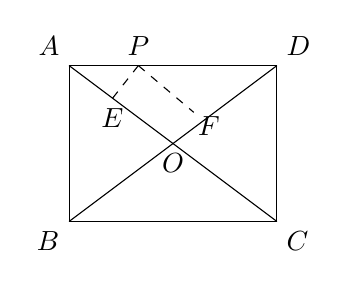
\begin{tikzpicture}[scale=0.22]
\draw (0,0) node[below left]{$B$} -- (12,0) node[below right]{$C$} -- (12,9) node[above right]{$D$} -- (0,9) node[above left]{$A$} -- cycle;
\draw (0,9) -- (12,0); \draw (0,0) -- (12,9);
\node[below] at (6,4.5) {$O$};
\coordinate (P) at (4,9); \node[above] at (P) {$P$};
\draw[dashed] (P) -- (2.5, 7.1) node[below]{$E$};
\draw[dashed] (P) -- (7.2, 6.3) node[below right=-2pt]{$F$};
\end{tikzpicture}
\end{minipage}
}

\Q{老师在黑板上写了若干个从 1 开始的连续自然数：$1, 2, 3, 4, \dots$，后来擦掉其中的一个，剩下的数的平均数是 $18\dfrac{3}{17}$，擦掉的自然数是\underline{\hspace{3em}}。}

\Q{快、慢两车同时从甲、乙两地相向开出，快车行完全程需 8 小时，慢车行完全程需 12 小时。两车在途中相遇后，快车又行了 88 千米，这时快车已行了全程的 $\dfrac{7}{8}$。甲、乙两地相距多少千米？}

\Q{一列火车出发 2 小时后因故停车 0.5 小时，然后以原速的 $\dfrac{5}{6}$ 前进，最终到达目的地晚 1.5 小时。若出发 2 小时后又前进 150 公里再因故停车 0.5 小时，然后同样以原速的 $\dfrac{5}{6}$ 前进，则到达目的地仅晚 1 小时。那么整个路程为多少公里？}

\Qlast{将长方体石块（长$a$、宽$b$、高$c$，且 $a>b>c$）放入一圆柱形水槽内，并向水槽内匀速注水，速度为 $v \text{ cm}^3/\text{s}$，直至注满水槽为止。石块可以以三种不同的方式完全放入水槽内，如图1~图3所示。在这三种情况下，水槽内的水深 $h$ (cm) 与注水时间 $t$ (s) 的函数关系如图4~图6所示。

\vspace{-0.5em}
\begin{center}
\begin{tikzpicture}[scale=0.23]
  \draw (0,4) ellipse (3 and 0.8); \draw (-3,0) -- (-3,4); \draw (3,0) -- (3,4);
  \draw (-3,0) arc (180:360:3 and 0.8); \draw[dashed] (3,0) arc (0:180:3 and 0.8);
  \draw[fill=gray!30] (-1.5, -0.4) rectangle (1.5, 0.6); \draw[fill=gray!50] (1.5, -0.4) -- (2.2, 0) -- (2.2, 1) -- (1.5, 0.6) -- cycle; \draw[fill=gray!20] (-1.5, 0.6) -- (1.5, 0.6) -- (2.2, 1) -- (-0.8, 1) -- cycle; \node[below] at (0,-1.5) {图1};
\end{tikzpicture}
\hspace{0.5cm}
\begin{tikzpicture}[scale=0.23]
  \draw (0,4) ellipse (3 and 0.8); \draw (-3,0) -- (-3,4); \draw (3,0) -- (3,4);
  \draw (-3,0) arc (180:360:3 and 0.8); \draw[dashed] (3,0) arc (0:180:3 and 0.8);
  \draw[fill=gray!30] (-0.8, -0.6) rectangle (0.8, 3.5); \draw[fill=gray!50] (0.8, -0.6) -- (1.5, -0.2) -- (1.5, 3.9) -- (0.8, 3.5) -- cycle; \draw[fill=gray!20] (-0.8, 3.5) -- (0.8, 3.5) -- (1.5, 3.9) -- (-0.1, 3.9) -- cycle; \node[below] at (0,-1.5) {图2};
\end{tikzpicture}
\hspace{0.5cm}
\begin{tikzpicture}[scale=0.23]
  \draw (0,4) ellipse (3 and 0.8); \draw (-3,0) -- (-3,4); \draw (3,0) -- (3,4);
  \draw (-3,0) arc (180:360:3 and 0.8); \draw[dashed] (3,0) arc (0:180:3 and 0.8);
  \draw[fill=gray!30] (-1, -0.5) rectangle (1, 2.5); \draw[fill=gray!50] (1, -0.5) -- (1.8, -0.1) -- (1.8, 2.9) -- (1, 2.5) -- cycle; \draw[fill=gray!20] (-1, 2.5) -- (1, 2.5) -- (1.8, 2.9) -- (-0.2, 2.9) -- cycle; \node[below] at (0,-1.5) {图3};
\end{tikzpicture}
\end{center}
\vspace{-1.5em}
\begin{center}
\begin{tikzpicture}[scale=0.52]
  \draw[->] (-0.2,0) -- (3.5,0) node[right]{\scriptsize $t/\text{s}$}; \draw[->] (0,-0.2) -- (0,3) node[above]{\scriptsize $h/\text{cm}$}; \draw (0,0) node[below left]{\scriptsize $O$};
  \draw[thick] (0,0) -- (1.5, 1.2) node[above left=-2pt]{\scriptsize $A$} -- (2.8, 2.5) node[above]{\scriptsize $B$};
  \draw[dashed] (1.5,0) node[below]{\scriptsize 13} -- (1.5,1.2) -- (0,1.2) node[left]{\scriptsize 5};
  \draw[dashed] (2.8,0) node[below]{\scriptsize 69} -- (2.8,2.5) -- (0,2.5) node[left]{\scriptsize 12}; \node[below] at (1.5,-0.8) {图4};
\end{tikzpicture}
\hspace{0.3cm}
\begin{tikzpicture}[scale=0.52]
  \draw[->] (-0.2,0) -- (3.5,0) node[right]{\scriptsize $t/\text{s}$}; \draw[->] (0,-0.2) -- (0,3) node[above]{\scriptsize $h/\text{cm}$}; \draw (0,0) node[below left]{\scriptsize $O$};
  \draw[thick] (0,0) -- (2.2, 2.0) node[above left=-2pt]{\scriptsize $C$} -- (2.8, 2.5) node[above]{\scriptsize $D$};
  \draw[dashed] (2.2,0) node[below]{\scriptsize 45} -- (2.2,2.0) -- (0,2.0) node[left]{\scriptsize 9};
  \draw[dashed] (2.8,0) node[below]{\scriptsize 69} -- (2.8,2.5) -- (0,2.5) node[left]{\scriptsize 12}; \node[below] at (1.5,-0.8) {图5};
\end{tikzpicture}
\hspace{0.3cm}
\begin{tikzpicture}[scale=0.52]
  \draw[->] (-0.2,0) -- (3.5,0) node[right]{\scriptsize $t/\text{s}$}; \draw[->] (0,-0.2) -- (0,3) node[above]{\scriptsize $h/\text{cm}$}; \draw (0,0) node[below left]{\scriptsize $O$};
  \draw[thick] (0,0) -- (2.8, 2.5) node[above]{\scriptsize $E$};
  \draw[dashed] (2.8,0) node[below]{\scriptsize 69} -- (2.8,2.5) -- (0,2.5) node[left]{\scriptsize 12}; \node[below] at (1.5,-0.8) {图6};
\end{tikzpicture}
\end{center}
根据图象完成下列问题：\\
(1) 请分别将三种放置方式的示意图和与之对应的关系图象用线连接起来；\\
(2) 水槽的高\underline{\hspace{2em}}cm；石块的长 $a=$\underline{\hspace{2em}}cm；宽 $b=$\underline{\hspace{2em}}cm；高 $c=$\underline{\hspace{2em}}cm；\\
(3) 求圆柱形水槽的底面积 $S$（用含 $v$ 的式子表示）。}

\end{OnePageSixFill}

% =========================================================
% 7.21
% =========================================================
\section*{7月21日作业（6道题当晚22:00前打卡）}
\begin{OnePageSixFill}

\Q{解方程组：$\begin{cases} 2x + 3y = 16 \\ \dfrac{x-1}{2} = \dfrac{y+2}{2} \end{cases}$}

\Q{
\begin{minipage}[c]{0.75\textwidth}
在长方形 ABCD 中，已知两邻边 $AD=15$，$AB=8$，对角线 $AC=17$，$O$ 为对角线交点。$P$ 是 $AD$ 边上异于 $A$ 和 $D$ 的一个动点，过点 $P$ 分别向 $OA, OD$ 作垂线 $PE, PF$，那么 $PE+PF$ 有\underline{\hspace{3em}}值（最大、最小、定值），这个值为\underline{\hspace{3em}}。
\end{minipage}
\hfill
\begin{minipage}[c]{0.22\textwidth}
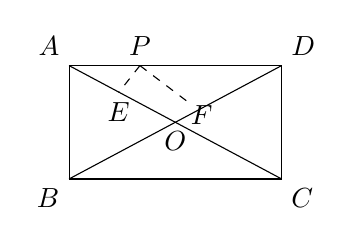
\begin{tikzpicture}[scale=0.18]
\draw (0,0) node[below left]{$B$} -- (15,0) node[below right]{$C$} -- (15,8) node[above right]{$D$} -- (0,8) node[above left]{$A$} -- cycle;
\draw (0,8) -- (15,0); \draw (0,0) -- (15,8);
\node[below] at (7.5,4) {$O$};
\coordinate (P) at (5,8); \node[above] at (P) {$P$};
\draw[dashed] (P) -- (3.5, 6.1) node[below]{$E$};
\draw[dashed] (P) -- (8.3, 5.5) node[below right=-2pt]{$F$};
\end{tikzpicture}
\end{minipage}
}

\Q{老师在黑板上写了若干个从 1 开始的连续自然数：$1, 2, 3, 4, \dots$，后来擦掉其中的一个，剩下的数的平均数是 $20\dfrac{5}{19}$，擦掉的自然数是\underline{\hspace{3em}}。}

\Q{快、慢两车同时从甲、乙两地相向开出，快车行完全程需 9 小时，慢车行完全程需 18 小时。两车在途中相遇后，快车又行了 60 千米，这时快车已行了全程的 $\dfrac{5}{6}$。甲、乙两地相距多少千米？}

\Q{一列火车出发 1.5 小时后因故停车 1 小时，然后以原速的 $\dfrac{2}{3}$ 前进，最终到达目的地晚 2.5 小时。若出发 1.5 小时后又前进 70 公里再因故停车 1 小时，然后同样以原速的 $\dfrac{2}{3}$ 前进，则到达目的地仅晚 2 小时。那么整个路程为多少公里？}

\Qlast{将长方体石块（长$a$、宽$b$、高$c$，且 $a>b>c$）放入一圆柱形水槽内，并向水槽内匀速注水，速度为 $v \text{ cm}^3/\text{s}$，直至注满水槽为止。石块可以以三种不同的方式完全放入水槽内。在这三种情况下，水深 $h$ (cm) 与注水时间 $t$ (s) 的函数关系如图4~图6所示。

\vspace{-0.5em}
\begin{center}
\begin{tikzpicture}[scale=0.52]
  \draw[->] (-0.2,0) -- (3.5,0) node[right]{\scriptsize $t/\text{s}$}; \draw[->] (0,-0.2) -- (0,3) node[above]{\scriptsize $h/\text{cm}$}; \draw (0,0) node[below left]{\scriptsize $O$};
  \draw[thick] (0,0) -- (1.5, 1.2) node[above left=-2pt]{\scriptsize $A$} -- (2.8, 2.5) node[above]{\scriptsize $B$};
  \draw[dashed] (1.5,0) node[below]{\scriptsize 32} -- (1.5,1.2) -- (0,1.2) node[left]{\scriptsize 8};
  \draw[dashed] (2.8,0) node[below]{\scriptsize 102} -- (2.8,2.5) -- (0,2.5) node[left]{\scriptsize 15}; \node[below] at (1.5,-0.8) {图4};
\end{tikzpicture}
\hspace{0.3cm}
\begin{tikzpicture}[scale=0.52]
  \draw[->] (-0.2,0) -- (3.5,0) node[right]{\scriptsize $t/\text{s}$}; \draw[->] (0,-0.2) -- (0,3) node[above]{\scriptsize $h/\text{cm}$}; \draw (0,0) node[below left]{\scriptsize $O$};
  \draw[thick] (0,0) -- (2.2, 2.0) node[above left=-2pt]{\scriptsize $C$} -- (2.8, 2.5) node[above]{\scriptsize $D$};
  \draw[dashed] (2.2,0) node[below]{\scriptsize 72} -- (2.2,2.0) -- (0,2.0) node[left]{\scriptsize 12};
  \draw[dashed] (2.8,0) node[below]{\scriptsize 102} -- (2.8,2.5) -- (0,2.5) node[left]{\scriptsize 15}; \node[below] at (1.5,-0.8) {图5};
\end{tikzpicture}
\hspace{0.3cm}
\begin{tikzpicture}[scale=0.52]
  \draw[->] (-0.2,0) -- (3.5,0) node[right]{\scriptsize $t/\text{s}$}; \draw[->] (0,-0.2) -- (0,3) node[above]{\scriptsize $h/\text{cm}$}; \draw (0,0) node[below left]{\scriptsize $O$};
  \draw[thick] (0,0) -- (2.8, 2.5) node[above]{\scriptsize $E$};
  \draw[dashed] (2.8,0) node[below]{\scriptsize 102} -- (2.8,2.5) -- (0,2.5) node[left]{\scriptsize 15}; \node[below] at (1.5,-0.8) {图6};
\end{tikzpicture}
\end{center}
已知图1~图3的摆放方式同上题。(1) 请连线（略）；(2) 水槽的高\underline{\hspace{2em}}cm；石块的长 $a=$\underline{\hspace{2em}}cm；宽 $b=$\underline{\hspace{2em}}cm；高 $c=$\underline{\hspace{2em}}cm；(3) 求水槽底面积 $S$（用含 $v$ 的式子表示）。}

\end{OnePageSixFill}

% =========================================================
% 7.22
% =========================================================
\section*{7月22日作业（6道题当晚22:00前打卡）}
\begin{OnePageSixFill}

\Q{解方程组：$\begin{cases} 4x - y = 7 \\ \dfrac{x+1}{2} = \dfrac{y-1}{2} \end{cases}$}

\Q{
\begin{minipage}[c]{0.75\textwidth}
在长方形 ABCD 中，已知两邻边 $AD=24$，$AB=7$，对角线 $AC=25$，$O$ 为对角线交点。$P$ 是 $AD$ 边上异于 $A$ 和 $D$ 的一个动点，过点 $P$ 分别向 $OA, OD$ 作垂线 $PE, PF$，那么 $PE+PF$ 有\underline{\hspace{3em}}值（最大、最小、定值），这个值为\underline{\hspace{3em}}。
\end{minipage}
\hfill
\begin{minipage}[c]{0.22\textwidth}
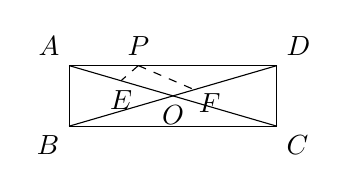
\begin{tikzpicture}[scale=0.11]
\draw (0,0) node[below left]{$B$} -- (24,0) node[below right]{$C$} -- (24,7) node[above right]{$D$} -- (0,7) node[above left]{$A$} -- cycle;
\draw (0,7) -- (24,0); \draw (0,0) -- (24,7);
\node[below] at (12,3.5) {$O$};
\coordinate (P) at (8,7); \node[above] at (P) {$P$};
\draw[dashed] (P) -- (6, 5.25) node[below]{$E$};
\draw[dashed] (P) -- (14.5, 4.2) node[below right=-2pt]{$F$};
\end{tikzpicture}
\end{minipage}
}

\Q{老师在黑板上写了若干个从 1 开始的连续自然数：$1, 2, 3, 4, \dots$，后来擦掉其中的一个，剩下的数的平均数是 $22\dfrac{8}{21}$，擦掉的自然数是\underline{\hspace{3em}}。}

\Q{快、慢两车同时从甲、乙两地相向开出，快车行完全程需 12 小时，慢车行完全程需 20 小时。两车在途中相遇后，快车又行了 110 千米，这时快车已行了全程的 $\dfrac{9}{10}$。甲、乙两地相距多少千米？}

\Q{一列火车出发 2.5 小时后因故停车 0.5 小时，然后以原速的 $\dfrac{3}{4}$ 前进，最终到达目的地晚 1.5 小时。若出发 2.5 小时后又前进 120 公里再因故停车 0.5 小时，然后同样以原速的 $\dfrac{3}{4}$ 前进，则到达目的地仅晚 1 小时。那么整个路程为多少公里？}

\Qlast{将长方体石块（长$a$、宽$b$、高$c$，且 $a>b>c$）放入一圆柱形水槽内，并向水槽内匀速注水，速度为 $v \text{ cm}^3/\text{s}$，直至注满水槽为止。石块可以以三种不同的方式完全放入水槽内。在这三种情况下，水深 $h$ (cm) 与注水时间 $t$ (s) 的函数关系如图4~图6所示。

\vspace{-0.5em}
\begin{center}
\begin{tikzpicture}[scale=0.52]
  \draw[->] (-0.2,0) -- (3.5,0) node[right]{\scriptsize $t/\text{s}$}; \draw[->] (0,-0.2) -- (0,3) node[above]{\scriptsize $h/\text{cm}$}; \draw (0,0) node[below left]{\scriptsize $O$};
  \draw[thick] (0,0) -- (1.5, 1.2) node[above left=-2pt]{\scriptsize $A$} -- (2.8, 2.5) node[above]{\scriptsize $B$};
  \draw[dashed] (1.5,0) node[below]{\scriptsize 18} -- (1.5,1.2) -- (0,1.2) node[left]{\scriptsize 5};
  \draw[dashed] (2.8,0) node[below]{\scriptsize 128} -- (2.8,2.5) -- (0,2.5) node[left]{\scriptsize 16}; \node[below] at (1.5,-0.8) {图4};
\end{tikzpicture}
\hspace{0.3cm}
\begin{tikzpicture}[scale=0.52]
  \draw[->] (-0.2,0) -- (3.5,0) node[right]{\scriptsize $t/\text{s}$}; \draw[->] (0,-0.2) -- (0,3) node[above]{\scriptsize $h/\text{cm}$}; \draw (0,0) node[below left]{\scriptsize $O$};
  \draw[thick] (0,0) -- (2.2, 2.0) node[above left=-2pt]{\scriptsize $C$} -- (2.8, 2.5) node[above]{\scriptsize $D$};
  \draw[dashed] (2.2,0) node[below]{\scriptsize 68} -- (2.2,2.0) -- (0,2.0) node[left]{\scriptsize 10};
  \draw[dashed] (2.8,0) node[below]{\scriptsize 128} -- (2.8,2.5) -- (0,2.5) node[left]{\scriptsize 16}; \node[below] at (1.5,-0.8) {图5};
\end{tikzpicture}
\hspace{0.3cm}
\begin{tikzpicture}[scale=0.52]
  \draw[->] (-0.2,0) -- (3.5,0) node[right]{\scriptsize $t/\text{s}$}; \draw[->] (0,-0.2) -- (0,3) node[above]{\scriptsize $h/\text{cm}$}; \draw (0,0) node[below left]{\scriptsize $O$};
  \draw[thick] (0,0) -- (2.8, 2.5) node[above]{\scriptsize $E$};
  \draw[dashed] (2.8,0) node[below]{\scriptsize 128} -- (2.8,2.5) -- (0,2.5) node[left]{\scriptsize 16}; \node[below] at (1.5,-0.8) {图6};
\end{tikzpicture}
\end{center}
已知图1~图3的摆放方式同第一天。(1) 请连线（略）；(2) 水槽的高\underline{\hspace{2em}}cm；石块的长 $a=$\underline{\hspace{2em}}cm；宽 $b=$\underline{\hspace{2em}}cm；高 $c=$\underline{\hspace{2em}}cm；(3) 求水槽底面积 $S$（用含 $v$ 的式子表示）。}

\end{OnePageSixFill}

% =========================================================
% 7.23
% =========================================================
\section*{7月23日作业（6道题当晚22:00前打卡）}
\begin{OnePageSixFill}

\Q{解方程组：$\begin{cases} x + 2y = 14 \\ \dfrac{x-2}{2} = \dfrac{y+2}{3} \end{cases}$}

\Q{
\begin{minipage}[c]{0.75\textwidth}
在长方形 ABCD 中，已知两邻边 $AD=24$，$AB=10$，对角线 $AC=26$，$O$ 为对角线交点。$P$ 是 $AD$ 边上异于 $A$ 和 $D$ 的一个动点，过点 $P$ 分别向 $OA, OD$ 作垂线 $PE, PF$，那么 $PE+PF$ 有\underline{\hspace{3em}}值（最大、最小、定值），这个值为\underline{\hspace{3em}}。
\end{minipage}
\hfill
\begin{minipage}[c]{0.22\textwidth}
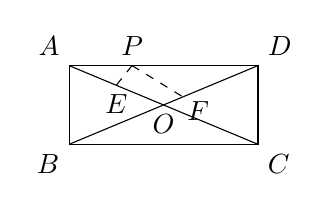
\begin{tikzpicture}[scale=0.1]
\draw (0,0) node[below left]{$B$} -- (24,0) node[below right]{$C$} -- (24,10) node[above right]{$D$} -- (0,10) node[above left]{$A$} -- cycle;
\draw (0,10) -- (24,0); \draw (0,0) -- (24,10);
\node[below] at (12,5) {$O$};
\coordinate (P) at (8,10); \node[above] at (P) {$P$};
\draw[dashed] (P) -- (6, 7.5) node[below]{$E$};
\draw[dashed] (P) -- (14.5, 6.0) node[below right=-2pt]{$F$};
\end{tikzpicture}
\end{minipage}
}

\Q{老师在黑板上写了若干个从 1 开始的连续自然数：$1, 2, 3, 4, \dots$，后来擦掉其中的一个，剩下的数的平均数是 $14\dfrac{3}{13}$，擦掉的自然数是\underline{\hspace{3em}}。}

\Q{快、慢两车同时从甲、乙两地相向开出，快车行完全程需 10 小时，慢车行完全程需 15 小时。两车在途中相遇后，快车又行了 70 千米，这时快车已行了全程的 $\dfrac{5}{6}$。甲、乙两地相距多少千米？}

\Q{一列火车出发 1 小时后因故停车 1.5 小时，然后以原速的 $\dfrac{4}{5}$ 前进，最终到达目的地晚 2.5 小时。若出发 1 小时后又前进 180 公里再因故停车 1.5 小时，然后同样以原速的 $\dfrac{4}{5}$ 前进，则到达目的地仅晚 2 小时。那么整个路程为多少公里？}

\Qlast{将长方体石块（长$a$、宽$b$、高$c$，且 $a>b>c$）放入一圆柱形水槽内，并向水槽内匀速注水，速度为 $v \text{ cm}^3/\text{s}$，直至注满水槽为止。在这三种情况下，水深 $h$ (cm) 与注水时间 $t$ (s) 的函数关系如图4~图6所示。

\vspace{-0.5em}
\begin{center}
\begin{tikzpicture}[scale=0.52]
  \draw[->] (-0.2,0) -- (3.5,0) node[right]{\scriptsize $t/\text{s}$}; \draw[->] (0,-0.2) -- (0,3) node[above]{\scriptsize $h/\text{cm}$}; \draw (0,0) node[below left]{\scriptsize $O$};
  \draw[thick] (0,0) -- (1.5, 1.2) node[above left=-2pt]{\scriptsize $A$} -- (2.8, 2.5) node[above]{\scriptsize $B$};
  \draw[dashed] (1.5,0) node[below]{\scriptsize 45} -- (1.5,1.2) -- (0,1.2) node[left]{\scriptsize 10};
  \draw[dashed] (2.8,0) node[below]{\scriptsize 165} -- (2.8,2.5) -- (0,2.5) node[left]{\scriptsize 20}; \node[below] at (1.5,-0.8) {图4};
\end{tikzpicture}
\hspace{0.3cm}
\begin{tikzpicture}[scale=0.52]
  \draw[->] (-0.2,0) -- (3.5,0) node[right]{\scriptsize $t/\text{s}$}; \draw[->] (0,-0.2) -- (0,3) node[above]{\scriptsize $h/\text{cm}$}; \draw (0,0) node[below left]{\scriptsize $O$};
  \draw[thick] (0,0) -- (2.2, 2.0) node[above left=-2pt]{\scriptsize $C$} -- (2.8, 2.5) node[above]{\scriptsize $D$};
  \draw[dashed] (2.2,0) node[below]{\scriptsize 105} -- (2.2,2.0) -- (0,2.0) node[left]{\scriptsize 15};
  \draw[dashed] (2.8,0) node[below]{\scriptsize 165} -- (2.8,2.5) -- (0,2.5) node[left]{\scriptsize 20}; \node[below] at (1.5,-0.8) {图5};
\end{tikzpicture}
\hspace{0.3cm}
\begin{tikzpicture}[scale=0.52]
  \draw[->] (-0.2,0) -- (3.5,0) node[right]{\scriptsize $t/\text{s}$}; \draw[->] (0,-0.2) -- (0,3) node[above]{\scriptsize $h/\text{cm}$}; \draw (0,0) node[below left]{\scriptsize $O$};
  \draw[thick] (0,0) -- (2.8, 2.5) node[above]{\scriptsize $E$};
  \draw[dashed] (2.8,0) node[below]{\scriptsize 165} -- (2.8,2.5) -- (0,2.5) node[left]{\scriptsize 20}; \node[below] at (1.5,-0.8) {图6};
\end{tikzpicture}
\end{center}
已知图1~图3的摆放方式同第一天。(1) 请连线（略）；(2) 水槽的高\underline{\hspace{2em}}cm；石块的长 $a=$\underline{\hspace{2em}}cm；宽 $b=$\underline{\hspace{2em}}cm；高 $c=$\underline{\hspace{2em}}cm；(3) 求水槽底面积 $S$（用含 $v$ 的式子表示）。}

\end{OnePageSixFill}

% =========================================================
% 7.24
% =========================================================
\section*{7月24日作业（6道题当晚22:00前打卡）}
\begin{OnePageSixFill}

\Q{解方程组：$\begin{cases} 5x - 3y = 5 \\ \dfrac{x-1}{3} = \dfrac{y-2}{3} \end{cases}$}

\Q{
\begin{minipage}[c]{0.75\textwidth}
在长方形 ABCD 中，已知两邻边 $AD=20$，$AB=15$，$AC=25$，$O$ 为交点。$P$ 是 $AD$ 边上异于 $A, D$ 的一个动点，过点 $P$ 分别向 $OA, OD$ 作垂线 $PE, PF$，那么 $PE+PF$ 有\underline{\hspace{3em}}值（最大、最小、定值），值为\underline{\hspace{3em}}。
\end{minipage}
\hfill
\begin{minipage}[c]{0.22\textwidth}
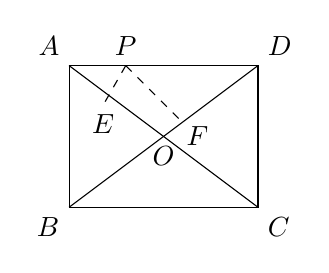
\begin{tikzpicture}[scale=0.12]
\draw (0,0) node[below left]{$B$} -- (20,0) node[below right]{$C$} -- (20,15) node[above right]{$D$} -- (0,15) node[above left]{$A$} -- cycle;
\draw (0,15) -- (20,0); \draw (0,0) -- (20,15);
\node[below] at (10,7.5) {$O$};
\coordinate (P) at (6,15); \node[above] at (P) {$P$};
\draw[dashed] (P) -- (3.6, 10.8) node[below]{$E$};
\draw[dashed] (P) -- (12, 9) node[below right=-2pt]{$F$};
\end{tikzpicture}
\end{minipage}
}

\Q{老师在黑板上写了若干个从 1 开始的连续自然数：$1, 2, 3, 4, \dots$，后来擦掉其中的一个，剩下的数的平均数是 $27\dfrac{3}{13}$，擦掉的自然数是\underline{\hspace{3em}}。}

\Q{快、慢两车同时从甲、乙两地相向开出，快车行完全程需 15 小时，慢车行完全程需 30 小时。两车在途中相遇后，快车又行了 100 千米，这时快车已行了全程的 $\dfrac{8}{9}$。甲、乙两地相距多少千米？}

\Q{一列火车出发 3 小时后因故停车 1 小时，然后以原速的 $\dfrac{5}{6}$ 前进，最终到达目的地晚 2 小时。若出发 3 小时后又前进 250 公里再因故停车 1 小时，然后同样以原速的 $\dfrac{5}{6}$ 前进，则到达目的地仅晚 1.5 小时。那么整个路程为多少公里？}

\Qlast{将长方体石块（长$a$、宽$b$、高$c$，且 $a>b>c$）放入一圆柱形水槽内，并向水槽内匀速注水，速度为 $v \text{ cm}^3/\text{s}$，直至注满水槽为止。在这三种情况下，水深 $h$ (cm) 与注水时间 $t$ (s) 的函数关系如图4~图6所示。

\vspace{-0.5em}
\begin{center}
\begin{tikzpicture}[scale=0.52]
  \draw[->] (-0.2,0) -- (3.5,0) node[right]{\scriptsize $t/\text{s}$}; \draw[->] (0,-0.2) -- (0,3) node[above]{\scriptsize $h/\text{cm}$}; \draw (0,0) node[below left]{\scriptsize $O$};
  \draw[thick] (0,0) -- (1.5, 1.2) node[above left=-2pt]{\scriptsize $A$} -- (2.8, 2.5) node[above]{\scriptsize $B$};
  \draw[dashed] (1.5,0) node[below]{\scriptsize 24} -- (1.5,1.2) -- (0,1.2) node[left]{\scriptsize 6};
  \draw[dashed] (2.8,0) node[below]{\scriptsize 144} -- (2.8,2.5) -- (0,2.5) node[left]{\scriptsize 18}; \node[below] at (1.5,-0.8) {图4};
\end{tikzpicture}
\hspace{0.3cm}
\begin{tikzpicture}[scale=0.52]
  \draw[->] (-0.2,0) -- (3.5,0) node[right]{\scriptsize $t/\text{s}$}; \draw[->] (0,-0.2) -- (0,3) node[above]{\scriptsize $h/\text{cm}$}; \draw (0,0) node[below left]{\scriptsize $O$};
  \draw[thick] (0,0) -- (2.2, 2.0) node[above left=-2pt]{\scriptsize $C$} -- (2.8, 2.5) node[above]{\scriptsize $D$};
  \draw[dashed] (2.2,0) node[below]{\scriptsize 84} -- (2.2,2.0) -- (0,2.0) node[left]{\scriptsize 12};
  \draw[dashed] (2.8,0) node[below]{\scriptsize 144} -- (2.8,2.5) -- (0,2.5) node[left]{\scriptsize 18}; \node[below] at (1.5,-0.8) {图5};
\end{tikzpicture}
\hspace{0.3cm}
\begin{tikzpicture}[scale=0.52]
  \draw[->] (-0.2,0) -- (3.5,0) node[right]{\scriptsize $t/\text{s}$}; \draw[->] (0,-0.2) -- (0,3) node[above]{\scriptsize $h/\text{cm}$}; \draw (0,0) node[below left]{\scriptsize $O$};
  \draw[thick] (0,0) -- (2.8, 2.5) node[above]{\scriptsize $E$};
  \draw[dashed] (2.8,0) node[below]{\scriptsize 144} -- (2.8,2.5) -- (0,2.5) node[left]{\scriptsize 18}; \node[below] at (1.5,-0.8) {图6};
\end{tikzpicture}
\end{center}
已知图1~图3的摆放方式同第一天。(1) 请连线（略）；(2) 水槽的高\underline{\hspace{2em}}cm；石块的长 $a=$\underline{\hspace{2em}}cm；宽 $b=$\underline{\hspace{2em}}cm；高 $c=$\underline{\hspace{2em}}cm；(3) 求水槽底面积 $S$（用含 $v$ 的式子表示）。}

\end{OnePageSixFill}

% =========================================================
% 7.25
% =========================================================
\section*{7月25日作业（6道题当晚22:00前打卡）}
\begin{OnePageSixFill}

\Q{解方程组：$\begin{cases} 3x + y = 12 \\ \dfrac{x+2}{2} = \dfrac{y-2}{2} \end{cases}$}

\Q{
\begin{minipage}[c]{0.75\textwidth}
在长方形 ABCD 中，已知两邻边 $AD=24$，$AB=18$，$AC=30$，$O$ 为交点。$P$ 是 $AD$ 边上异于 $A, D$ 的一个动点，过点 $P$ 分别向 $OA, OD$ 作垂线 $PE, PF$，那么 $PE+PF$ 有\underline{\hspace{3em}}值（最大、最小、定值），值为\underline{\hspace{3em}}。
\end{minipage}
\hfill
\begin{minipage}[c]{0.22\textwidth}
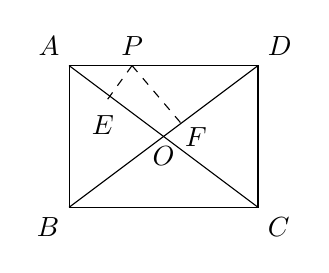
\begin{tikzpicture}[scale=0.1]
\draw (0,0) node[below left]{$B$} -- (24,0) node[below right]{$C$} -- (24,18) node[above right]{$D$} -- (0,18) node[above left]{$A$} -- cycle;
\draw (0,18) -- (24,0); \draw (0,0) -- (24,18);
\node[below] at (12,9) {$O$};
\coordinate (P) at (8,18); \node[above] at (P) {$P$};
\draw[dashed] (P) -- (4.3, 12.9) node[below]{$E$};
\draw[dashed] (P) -- (14.2, 10.7) node[below right=-2pt]{$F$};
\end{tikzpicture}
\end{minipage}
}

\Q{老师在黑板上写了若干个从 1 开始的连续自然数：$1, 2, 3, 4, \dots$，后来擦掉其中的一个，剩下的数的平均数是 $19\dfrac{1}{3}$，擦掉的自然数是\underline{\hspace{3em}}。}

\Q{快、慢两车同时从甲、乙两地相向开出，快车行完全程需 14 小时，慢车行完全程需 35 小时。两车在途中相遇后，快车又行了 85 千米，这时快车已行了全程的 $\dfrac{11}{12}$。甲、乙两地相距多少千米？}

\Q{一列火车出发 1 小时后因故停车 0.5 小时，然后以原速的 $\dfrac{2}{3}$ 前进，最终到达目的地晚 2 小时。若出发 1 小时后又前进 60 公里再因故停车 0.5 小时，然后同样以原速的 $\dfrac{2}{3}$ 前进，则到达目的地仅晚 1.5 小时。那么整个路程为多少公里？}

\Qlast{将长方体石块（长$a$、宽$b$、高$c$，且 $a>b>c$）放入一圆柱形水槽内，并向水槽内匀速注水，速度为 $v \text{ cm}^3/\text{s}$，直至注满水槽为止。在这三种情况下，水深 $h$ (cm) 与注水时间 $t$ (s) 的函数关系如图4~图6所示。

\vspace{-0.5em}
\begin{center}
\begin{tikzpicture}[scale=0.52]
  \draw[->] (-0.2,0) -- (3.5,0) node[right]{\scriptsize $t/\text{s}$}; \draw[->] (0,-0.2) -- (0,3) node[above]{\scriptsize $h/\text{cm}$}; \draw (0,0) node[below left]{\scriptsize $O$};
  \draw[thick] (0,0) -- (1.5, 1.2) node[above left=-2pt]{\scriptsize $A$} -- (2.8, 2.5) node[above]{\scriptsize $B$};
  \draw[dashed] (1.5,0) node[below]{\scriptsize 20} -- (1.5,1.2) -- (0,1.2) node[left]{\scriptsize 5};
  \draw[dashed] (2.8,0) node[below]{\scriptsize 60} -- (2.8,2.5) -- (0,2.5) node[left]{\scriptsize 10}; \node[below] at (1.5,-0.8) {图4};
\end{tikzpicture}
\hspace{0.3cm}
\begin{tikzpicture}[scale=0.52]
  \draw[->] (-0.2,0) -- (3.5,0) node[right]{\scriptsize $t/\text{s}$}; \draw[->] (0,-0.2) -- (0,3) node[above]{\scriptsize $h/\text{cm}$}; \draw (0,0) node[below left]{\scriptsize $O$};
  \draw[thick] (0,0) -- (2.2, 2.0) node[above left=-2pt]{\scriptsize $C$} -- (2.8, 2.5) node[above]{\scriptsize $D$};
  \draw[dashed] (2.2,0) node[below]{\scriptsize 44} -- (2.2,2.0) -- (0,2.0) node[left]{\scriptsize 8};
  \draw[dashed] (2.8,0) node[below]{\scriptsize 60} -- (2.8,2.5) -- (0,2.5) node[left]{\scriptsize 10}; \node[below] at (1.5,-0.8) {图5};
\end{tikzpicture}
\hspace{0.3cm}
\begin{tikzpicture}[scale=0.52]
  \draw[->] (-0.2,0) -- (3.5,0) node[right]{\scriptsize $t/\text{s}$}; \draw[->] (0,-0.2) -- (0,3) node[above]{\scriptsize $h/\text{cm}$}; \draw (0,0) node[below left]{\scriptsize $O$};
  \draw[thick] (0,0) -- (2.8, 2.5) node[above]{\scriptsize $E$};
  \draw[dashed] (2.8,0) node[below]{\scriptsize 60} -- (2.8,2.5) -- (0,2.5) node[left]{\scriptsize 10}; \node[below] at (1.5,-0.8) {图6};
\end{tikzpicture}
\end{center}
已知图1~图3的摆放方式同第一天。(1) 请连线（略）；(2) 水槽的高\underline{\hspace{2em}}cm；石块的长 $a=$\underline{\hspace{2em}}cm；宽 $b=$\underline{\hspace{2em}}cm；高 $c=$\underline{\hspace{2em}}cm；(3) 求水槽底面积 $S$（用含 $v$ 的式子表示）。}

\end{OnePageSixFill}

\end{document}